\documentclass{article} %[a4paper,10pt]
\usepackage[utf8]{inputenc}

\usepackage[english]{babel}

\usepackage{indentfirst}
\usepackage{multicol}
\usepackage{bbm}
\usepackage{amsmath}
\usepackage{amssymb}
% \usepackage{mathrsfs}
\usepackage{physics}
% \usepackage{calrsfs}
\usepackage{mathtools}
\usepackage{mathpunctspace}
\usepackage{wrapfig}

\usepackage[makeroom]{cancel}

\usepackage{graphicx}  % To include figures
\usepackage{subcaption}  % To use subfigure or subcaption environments


\usepackage{booktabs}

\usepackage{tikz}
\usepackage{pgfplots}
\usepackage{pgfplotstable}

\pgfplotsset{
    every axis plot/.append style={line width=0.5pt}
}

\usepackage{float}
\usepackage{hyperref}
\newfloat{graph}{htbp}{grp}
\floatname{graph}{Graf}

% Bibtex
\usepackage[
    %backend=biber, 
    natbib=true,
    style=numeric,
    sorting=none
]{biblatex}
% \usepackage{biblatex} %Imports biblatex package
\addbibresource{bibliography.bib} %Import the bibliography file
\usepackage{csquotes}

% \usepackage{algpseudocode}
\usepackage{algorithm, algorithmic}

\usepackage{xcolor}
\usepackage{graphicx} % path for gnuplot plots
\graphicspath{{graphics}}
\usepackage[top = 1cm, bottom = 1cm, left = 1cm, right = 1cm]{geometry}

\setlength{\textfloatsep}{1pt plus 1.0pt minus 2.0pt}

\title{Cahn-Hilliard model}
\author{Ján Kovačovský}


\pgfplotsset{compat=1.18}


\newcommand{\todo}[1]{\textcolor{red}{#1}}
\newcommand{\note}[1]{\textcolor{blue}{#1}}

\setcounter{section}{3}


\begin{document}

\section*{Cahn-Hilliard model}

The Cahn-Hilliard model can be formulated as a parabolic equation which is typically used to model phase separation in binary mixtures.
\begin{equation*}
    \partial_t c = \Delta \left(c^3 - c - \gamma \Delta c\right)
\end{equation*}

The order of this equation can be, however, lowered, yielding two coupled second-order partial differential evolution equations in terms of the so-called phase fraction $\phi$, which represents the concentration of one of the components in the binary mixture and the chemical potential $\mu$
\begin{equation}
    \frac{\partial \phi}{\partial t} = \nabla \cdot \left( b(\phi) \nabla \mu \right) \qq{and} \mu = -\gamma \Delta \phi + f'(\phi).
\end{equation}

The Time evolution $\partial_t \phi$ was approximated using Crank-Nicholson scheme. We studied the above system in a unit square $\Omega = (0, 1)^2$ with periodic boundary conditions, in other words, we were solving the system on a torus. The initial data for the phase fraction $\phi$ were given as\footnote{The values stated in the paper did not seem to correspond to the presented figures and so were adjusted in our simulations.}
\begin{equation}
    \phi_0 (x, y) = \cancelto{0.1}{0.3} \sin(4\pi x) \sin(2 \pi y) + \cancelto{0.6}{0.1}.
\end{equation}

The interface parameter $\gamma$ was set to $\gamma = 0.003$, the double well potential $f(\phi)$ and the mobility functions were defined as
\begin{equation}
    f(\phi) = 0.3 \left(\phi - 0.99\right)^2 \left(\phi + 0.99\right)^2 \qq{and} b(\phi) = \left(1 - \phi\right)^2 \left(1 + \phi\right)^2 + 10^{-3}.
\end{equation}

% The energy of this system, in constant time, can be calculated as
% \begin{equation}
%     \mathcal{E}(\phi) = \int_{\Omega} \frac{\gamma}{2} \left|\nabla \phi\right|^2 + f(\phi).
% \end{equation}

In order to solve the posed problem, we need to reformulate it first into the weak form
\begin{equation}
    \langle \partial_t \phi, v \rangle + \langle b(\phi) \nabla \mu, \nabla v \rangle = 0 \qq{and} \langle \mu - f'(\phi(t)), w \rangle - \langle \gamma \nabla \phi, \nabla w \rangle.
\end{equation}

As per the original article \cite{Brunk2023}, the model was computed with mixed elements and the Newton method was used to solve the corresponding \texttt{NonlinearVariationalProblem}.


Below we present the snapshots from the time evolution on the square as well as one instance of the model on a torus.


\begin{figure}[!h]
    \centering
    \begin{subfigure}[b]{0.2\textwidth}
        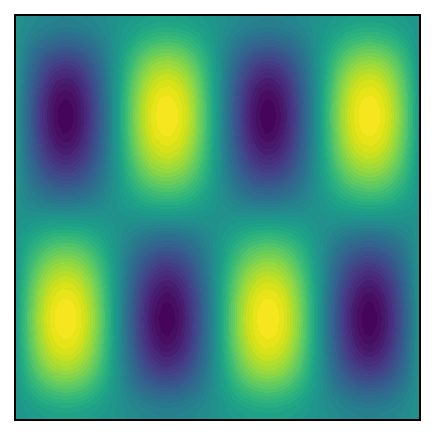
\includegraphics[width=\textwidth]{phi_0.pdf}
        \caption*{$t = 0$}
        \label{fig:image1}
    \end{subfigure}
    \hfill
    \begin{subfigure}[b]{0.2\textwidth}
        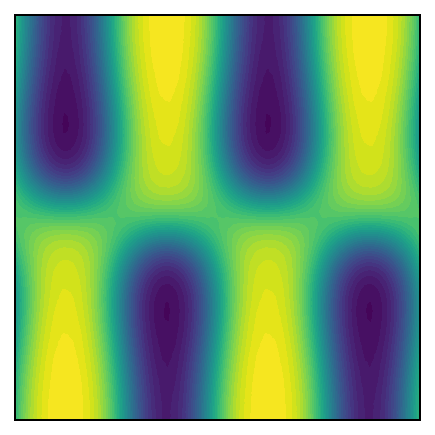
\includegraphics[width=\textwidth]{phi_0.05.pdf}
        \caption*{$t = 0.05$}
        \label{fig:image2}
    \end{subfigure}
    \hfill
    \begin{subfigure}[b]{0.2\textwidth}
        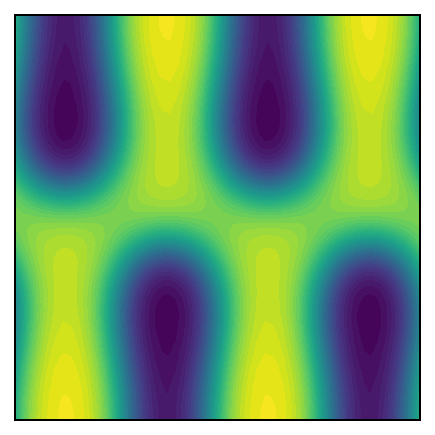
\includegraphics[width=\textwidth]{phi_0.1.pdf}
        \caption*{$t = 0.1$}
        \label{fig:image3}
    \end{subfigure}
    \hfill
    \begin{subfigure}[b]{0.2\textwidth}
        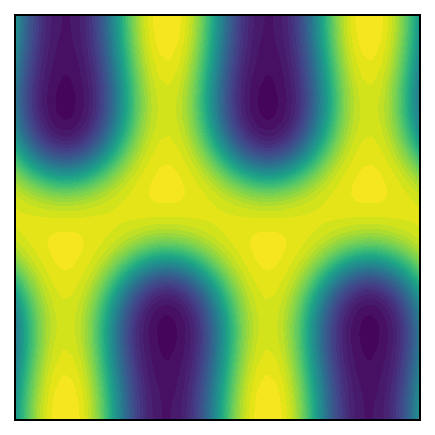
\includegraphics[width=\textwidth]{phi_0.2.pdf}
        \caption*{$t = 0.2$}
        \label{fig:image4}
    \end{subfigure}
    
    \vskip\baselineskip 
  
    \begin{subfigure}[b]{0.2\textwidth}
        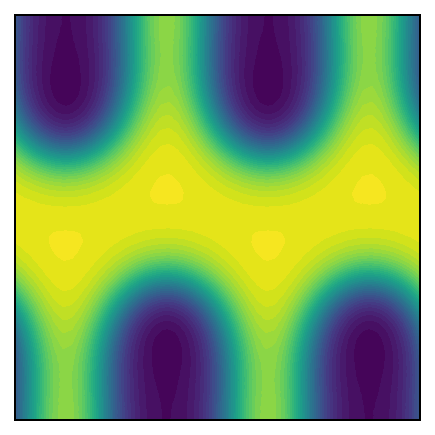
\includegraphics[width=\textwidth]{phi_0.3.pdf}
        \caption*{$t = 0.3$}
        \label{fig:image5}
    \end{subfigure}
    \hfill
    \begin{subfigure}[b]{0.2\textwidth}
        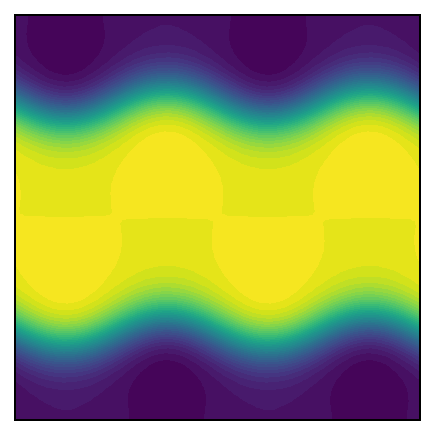
\includegraphics[width=\textwidth]{phi_0.4.pdf}
        \caption*{$t = 0.4$}
        \label{fig:image6}
    \end{subfigure}
    \hfill
    \begin{subfigure}[b]{0.2\textwidth}
        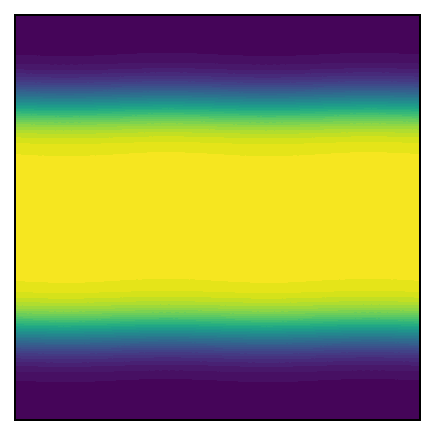
\includegraphics[width=\textwidth]{phi_0.5.pdf}
        \caption*{$t = 0.5$}
        \label{fig:image7}
    \end{subfigure}
    \hfill
    \begin{subfigure}[b]{0.2\textwidth}
        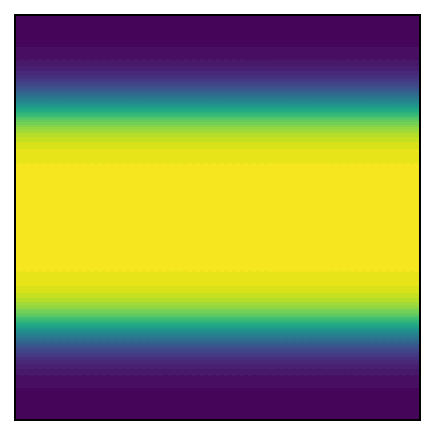
\includegraphics[width=\textwidth]{phi_1.pdf}
        \caption*{$t = 1$}
        \label{fig:image8}
    \end{subfigure}
    
    \caption{Snapshots from time evolution of the Cahn-Hilliard model on a unit square with periodic boundary conditions.}
    \label{fig:time-evolution}    
\end{figure}



% \begin{figure}[!h]
%     \centering
%     \begin{subfigure}[b]{0.2\textwidth}
%         \includegraphics[width=\textwidth]{square0.png}
%         \caption{$t = 0$}
%         \label{fig:image1}
%     \end{subfigure}
%     \hfill
%     \begin{subfigure}[b]{0.2\textwidth}
%         \includegraphics[width=\textwidth]{square1.png}
%         \caption{$t = 0.1$}
%         \label{fig:image2}
%     \end{subfigure}
%     \hfill
%     \begin{subfigure}[b]{0.2\textwidth}
%         \includegraphics[width=\textwidth]{square2.png}
%         \caption{$t = 0.2$}
%         \label{fig:image3}
%     \end{subfigure}
%     \hfill
%     \begin{subfigure}[b]{0.2\textwidth}
%         \includegraphics[width=\textwidth]{square3.png}
%         \caption{$t = 0.4$}
%         \label{fig:image4}
%     \end{subfigure}
%     \caption{Snapshots from time evolution of the Cahn-Hilliard model on a unit square with periodic boundary conditions.}
%     \label{fig:time-evolution}
% \end{figure}


\printbibliography

\end{document}
